\documentclass[11pt,letter,english]{article}
\usepackage{amssymb,babel,colortbl}
\usepackage{hyperref,rotating}
\usepackage{multirow}
\usepackage{color}
\providecommand{\href}[2]{#2}

\oddsidemargin=0mm
\evensidemargin=0mm
\textwidth=160mm
%\textwidth=170mm
%\textheight=232mm
\textheight=9.4in
%\textheight=287mm
\hoffset=0.5cm
%\hoffset=-1.6cm
%\voffset=-0.8cm
\voffset=-2.5cm
%\voffset=-2.4cm
%\documentclass[11pt,letter,english]{article}
%\usepackage{amssymb,babel,colortbl}
%\providecommand{\href}[2]{#2}   
%
%\oddsidemargin=0mm
%\evensidemargin=0mm
%\textwidth=160mm
%\textheight=9.4in
%\hoffset=-0.5cm
%\voffset=-1.2cm

\renewcommand\refname{Bibliography}  

\begin{document}
\nocite{*} 

\small
\newcommand*{\data}{\ifcase\month\or
  January\or February\or March\or April\or May\or June\or
  July\or August\or September\or October\or November\or December\fi
  \space\number\day th,\space\number\year}
%===============================================================================
% New Commands and Definitions
%===============================================================================
\newcommand{\blue}    {\color[named]{Blue}}
\newcommand{\black}   {\color[named]{Black}}
\newcommand{\red}     {\color[named]{Red}}
\newcommand{\green}   {\color[named]{Green}}
\newcommand{\orange}  {\color[named]{Orange}}
\newcommand{\yellow}  {\color[named]{Yellow}}
\newcommand{\magenta} {\color[named]{Magenta}}
\newcommand{\cyan}    {\color[named]{Cyan}}

\def\CP{{\sffamily CP}}

%===============================================================================
% Title
%===============================================================================
\begin{center}
 \section*{\huge{PS-Booster Ejection Correction Dipoles}} 
% \large \textbf{}
 \vspace {0.6cm}
\end{center}

%===============================================================================
% List Of Magnets
%===============================================================================
\subsection*{Goal}

Attempt to reproduce the results in http://wwwpsco.cern.ch/private/gm/gmdescrip/LINC-Note.pdf

\begin{itemize}
\item{Used the latest configuration files for {\bf Ring 3} from Vivien for the ring}
\item{{\bf Matched the optics in MADX (32 bits)} to get the tunes Q$_H=4.17$ and Q$_V=5.23$}
\item{After add a horizontal or vertical kick from one of the correction dipoles}
\item{Compare the closed orbit with the one from the note}
\item{Extract the geometrical relations between the kicks at the entry point and at the center of the ejection Septum, SMH15L1}
\item{Trying to use the 2014 configuration but moving dipole correctors and septum in the position mentioned in the note}
\end{itemize}



%===============================================================================
% Head-to-head Comparison
%===============================================================================
\subsection*{Head-to-head Comparison}

\begin{itemize}

\item Configuration 5: {\bf Expected from Note}
  \begin{itemize}
  \item center of DHZ,DVT 4L1 at=1.327-0.426 m = 0.901 m 
  \item center DHZ,DVT 11L1 at=1.327-0.950 m = 0.377 m 
  \item entrance of SMH15L1 4L1 at=1.327-0.8 m = 0.527 m 
  \end{itemize}
\end{itemize}


With the entrance of the septum we understood the beginning of the SMH15L1
septum blade.  From the drawing (thanks to M. Houricane), the blade does not
appear to be centered simmetrically w.r.t. the tank, but slightly shifted
upstream, see sketch in Figure~\ref{fig:smh15l1_simplified}. We Labeled {\bf A}
the distance between the beginning of the tank and the beginning of the
blade, {\bf B} the blade length, {\bf C} the distance between the end of the
blade and the end of the tank and {\bf X} the distance between the beginning of
the blade and the center of the tank. With some simple math one can deduct that:

\begin{equation}
X = \frac{B+C-A}{2}
\end{equation}

Using the values from drawing PS.CA.98411.1 of A=121.03 mm, B=1000.24 mm and
C=138.21 mm, one obtains X=508.706 mm. Thus if in the configuration expected from
the note one sets the SMH15L1 entrance to be at 0.527 m, this means the center
of SM15L1 is at (0.507+0.508706) m = 1.015706 m.

The results of using these values and a kick of 1 mrad are summarized in Table~\ref{tab:geom_rel}.

\begin{figure}[!hbtp]
  \begin{center}
    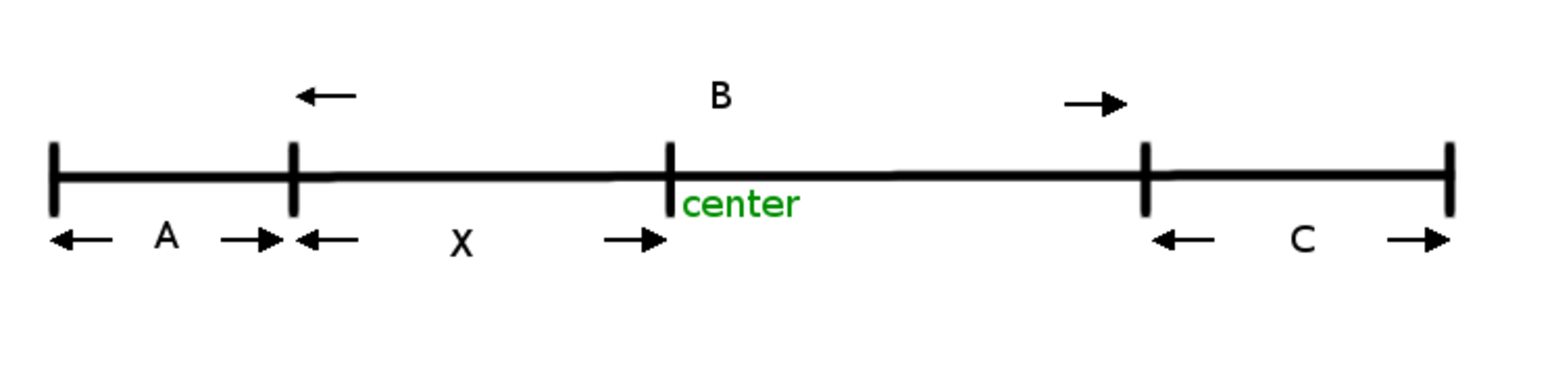
\includegraphics[width=1.0\textwidth]{figs/smh15l1.pdf}
    \caption{simplified drawing of SMH15L1. {\bf A} is the distance between the beginning of the tank and the beginning of the blade. {\bf B} is the blade length. 
      {\bf C} is the distance between the end of the blade and the end of the tank.}
    \label{fig:smh15l1_simplified}
  \end{center}
\end{figure}




\begin{table}[h]

  \caption{
    Comparison for the geometrical relation between the kicks in the different PSB sections at the entrance of SMH15L1
    }

  \label{tab:geom_rel}
%\hspace*{-1.3cm}

  \begin{tabular}{ |l|c|c| }\hline
  Kicker & Note Value  & Config. 5 \\ \hline
         & {\bf entrance of SMH15L1} & {\bf Beginning Blade} \\ \hline
  \multirow{2}{*}{BE3.DHZ4L1} & $\Delta$X$_{ES}$[mm]  = 0.760 $\cdot$ DHZ4L1 [mrad] & 0.786 \\  \cline{2-3}
                              & $\Delta$X'$_{ES}$[mm] = 0.947 $\cdot$ DHZ4L1 [mrad] & 0.938 \\  \hline      
  \multicolumn{3}{|c|}{}        \\ \hline

  \multirow{2}{*}{BE3.DHZ11L1} & $\Delta$X$_{ES}$[mm]  = 5.615 $\cdot$ DHZ11L1 [mrad] & 5.572 \\ \cline{2-3} 
                               & $\Delta$X'$_{ES}$[mm] = 0.104 $\cdot$ DHZ11L1 [mrad] & 0.105 \\ \hline      
 \multicolumn{3}{|c|}{} \\ \hline

 \multirow{2}{*}{BE3.DVT4L1} & $\Delta$Y$_{ES}$[mm]  = -2.122 $\cdot$ DVT4L1 [mrad] & -2.143 \\  \cline{2-3}  
                             & $\Delta$Y'$_{ES}$[mm] =  0.021 $\cdot$ DVT4L1 [mrad] &  0.023 \\  \hline       
 \multicolumn{3}{|c|}{} \\ \hline

 \multirow{2}{*}{BE3.DVT11L1} & $\Delta$Y$_{ES}$[mm]  =  0.669 $\cdot$ DVT11L1 [mrad] &  0.710 \\ \cline{2-3}  
                              & $\Delta$Y'$_{ES}$[mm] = -0.793 $\cdot$ DVT11L1 [mrad] & -0.798 \\ \hline       
 \multicolumn{3}{|c|}{} \\ \hline

\end{tabular}
\end{table}





%
%\begin{figure}[!hbtp]
%  \begin{center}
%    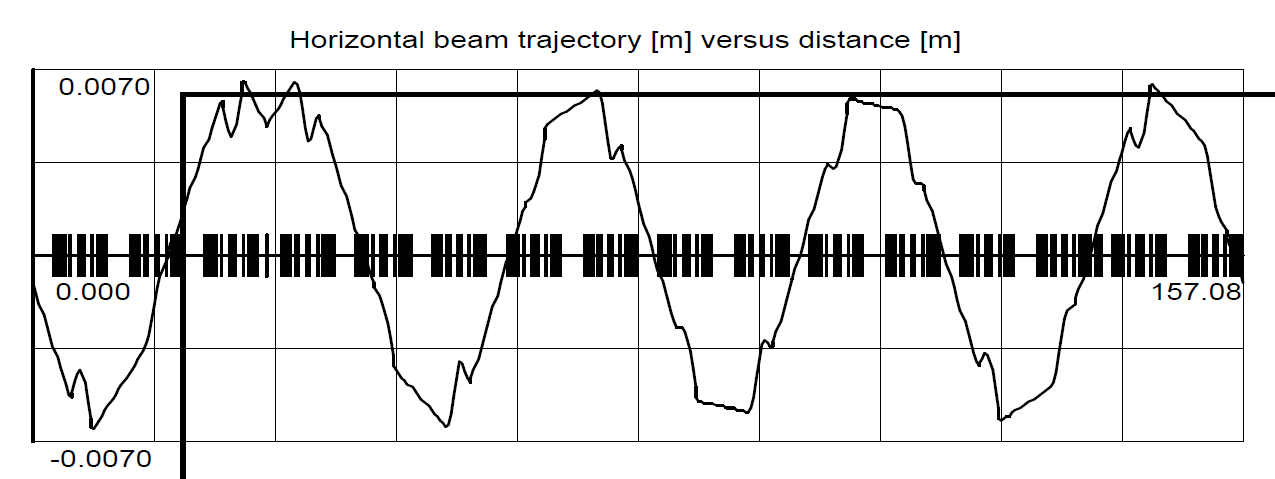
\includegraphics[width=1.0\textwidth]{figs/LINC-BE_DHZ4L1.png}
%    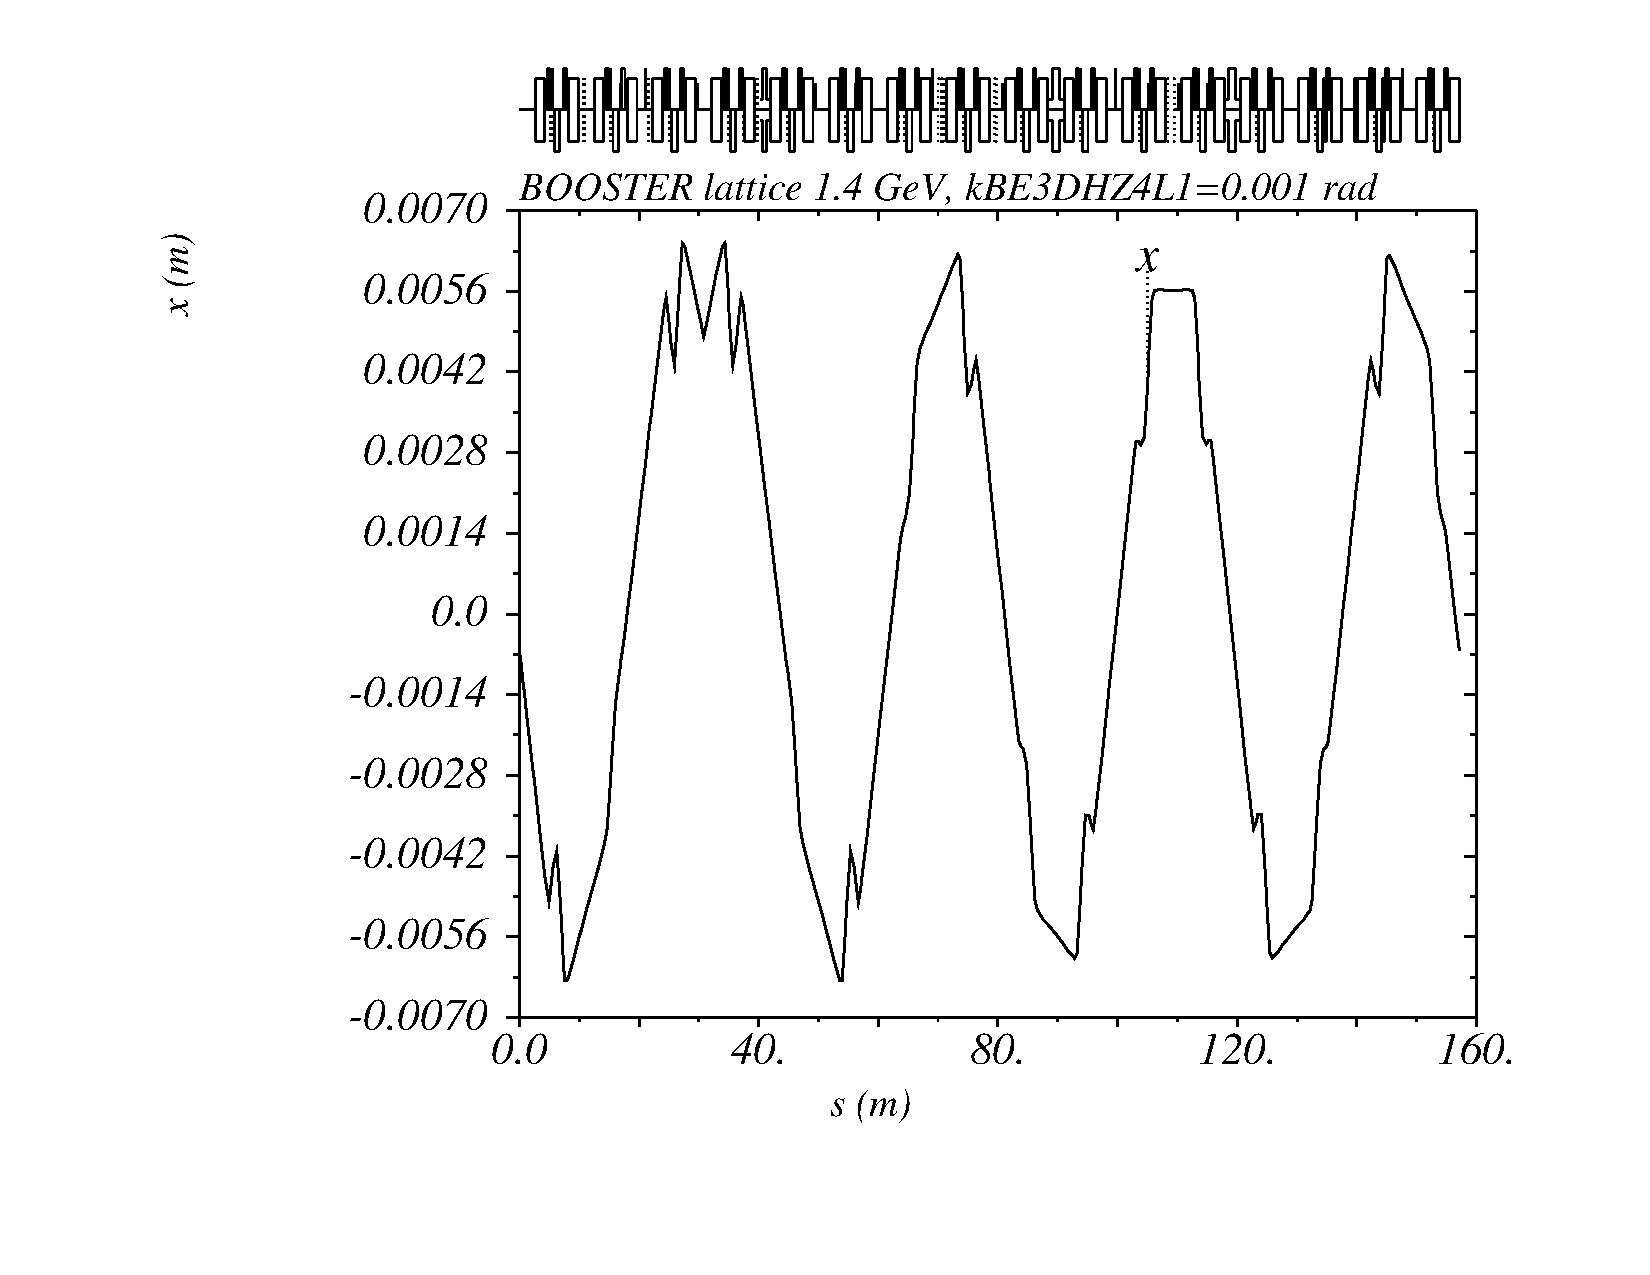
\includegraphics[width=1.0\textwidth]{figs/psb_orbit_BE3DHZ4L1at1mrad.pdf}
%    \caption{Closed Orbit comparison for a kick of 1 mrad for BE3.DHZ4L1. Top: from the note PS/OP/Note 99-xx of M. Benedikt. Bottom: Private MADX files}
%    \label{fig:BE_DHZ4L1}
%  \end{center}
%\end{figure}
%
%
%\begin{figure}[!hbtp]
%  \begin{center}
%    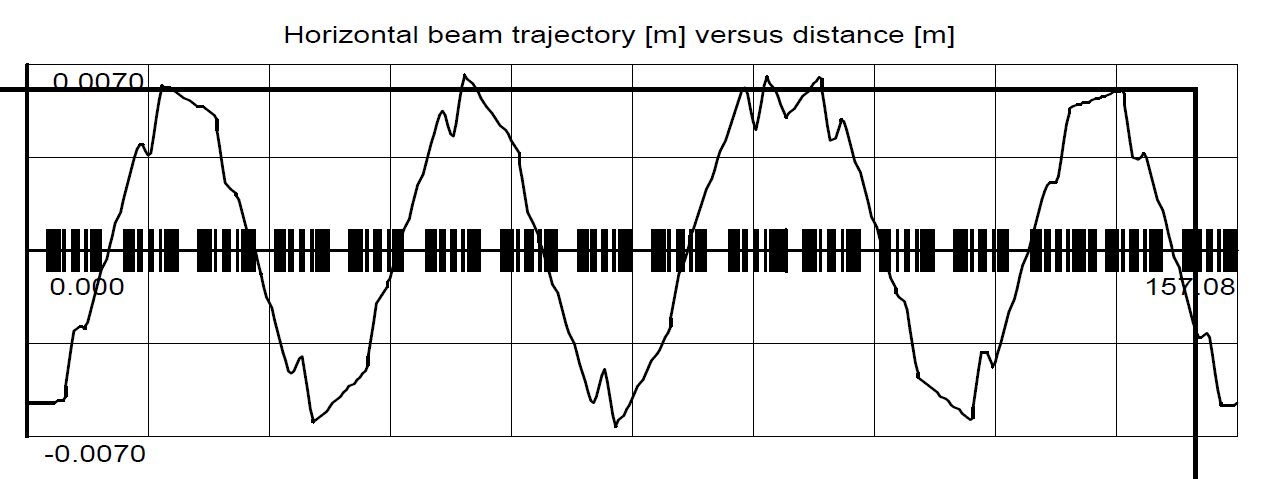
\includegraphics[width=1.0\textwidth]{figs/LINC-BE_DHZ11L1.png}
%    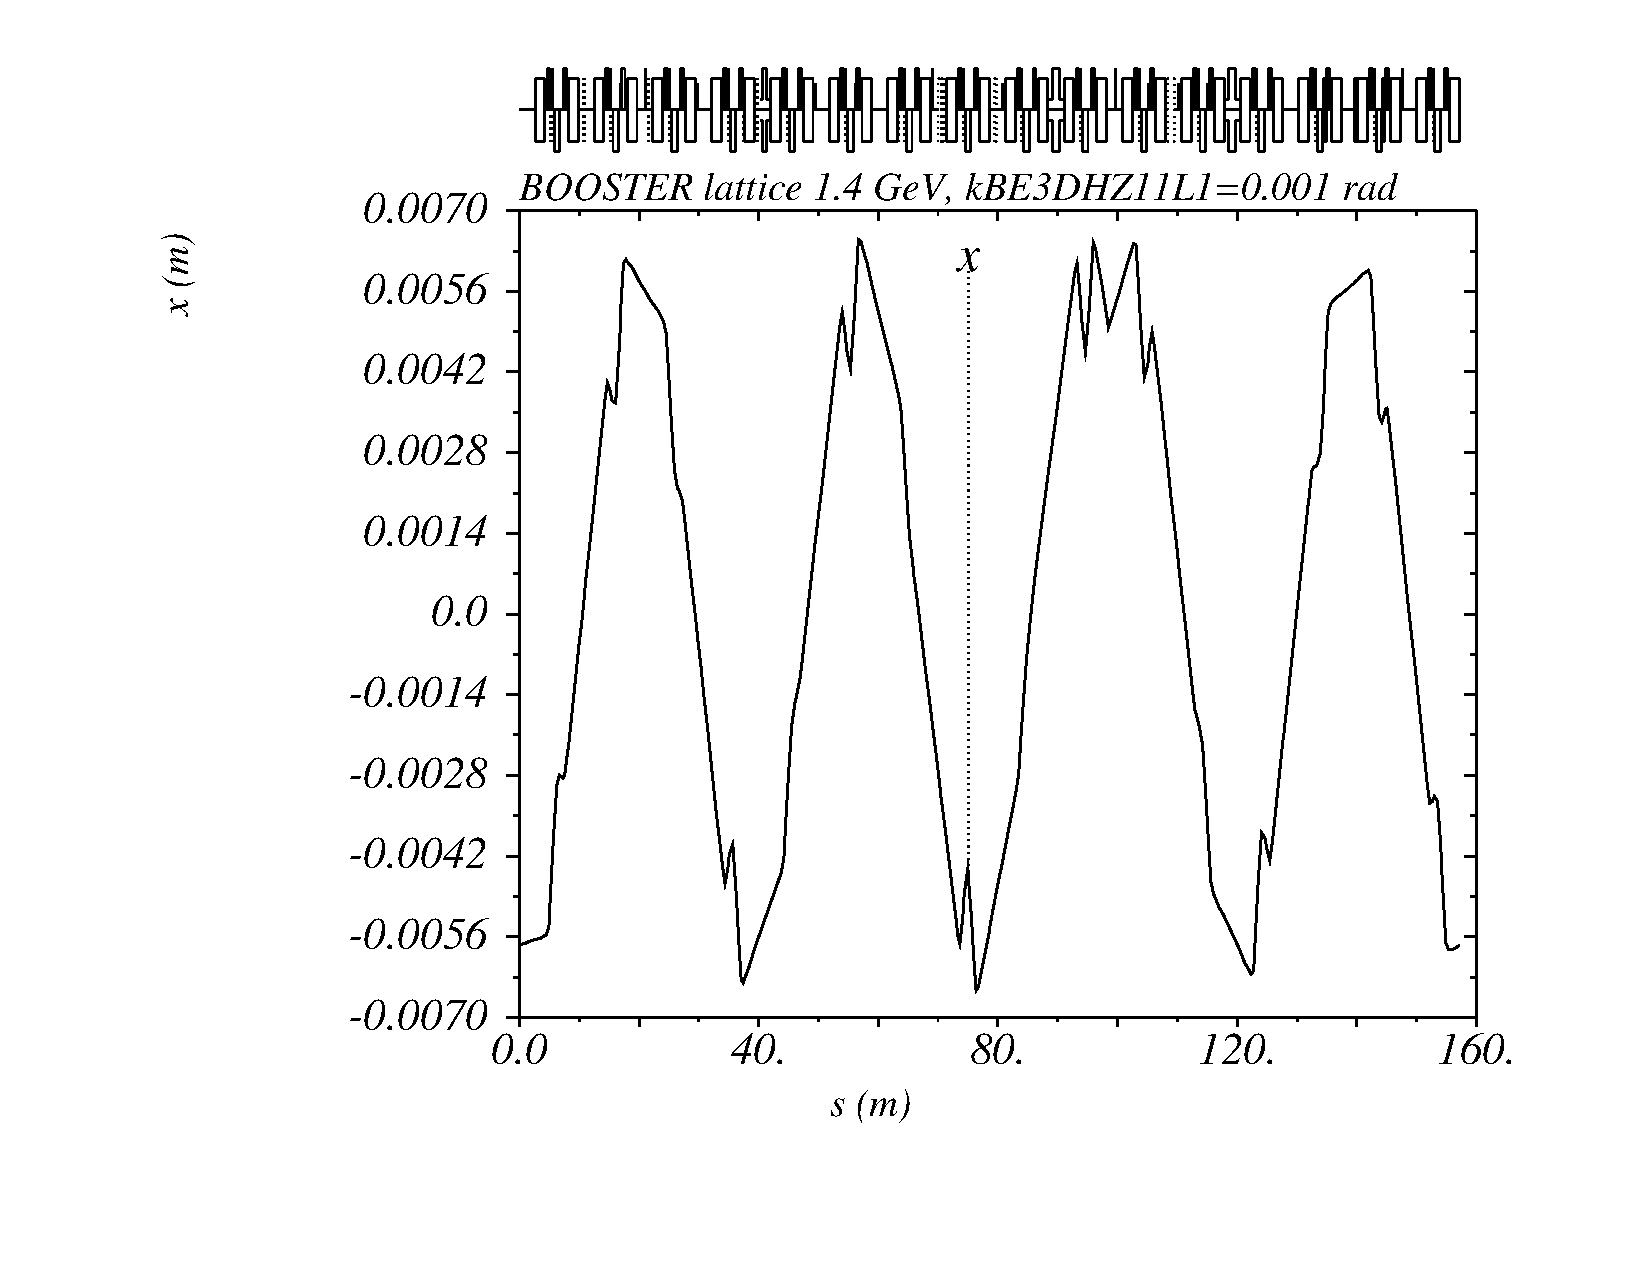
\includegraphics[width=1.0\textwidth]{figs/psb_orbit_BE3DHZ11L1at1mrad.pdf}
%    \caption{Closed Orbit comparison for a kick of 1 mrad for BE3.DHZ11L1. Top: from the note PS/OP/Note 99-xx of M. Benedikt. Bottom: Private MADX files}
%    \label{fig:BE_DHZ11L1}
%  \end{center}
%\end{figure}
%
%
%\begin{figure}[!hbtp]
%  \begin{center}
%    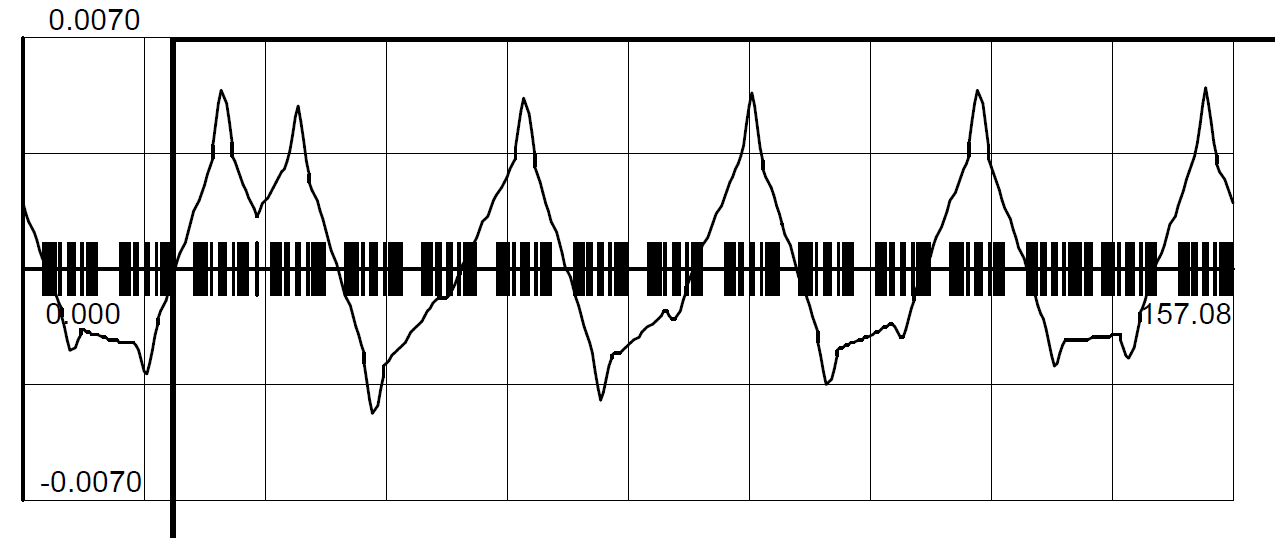
\includegraphics[width=1.0\textwidth]{figs/LINC-BE_DVT4L1.png}
%    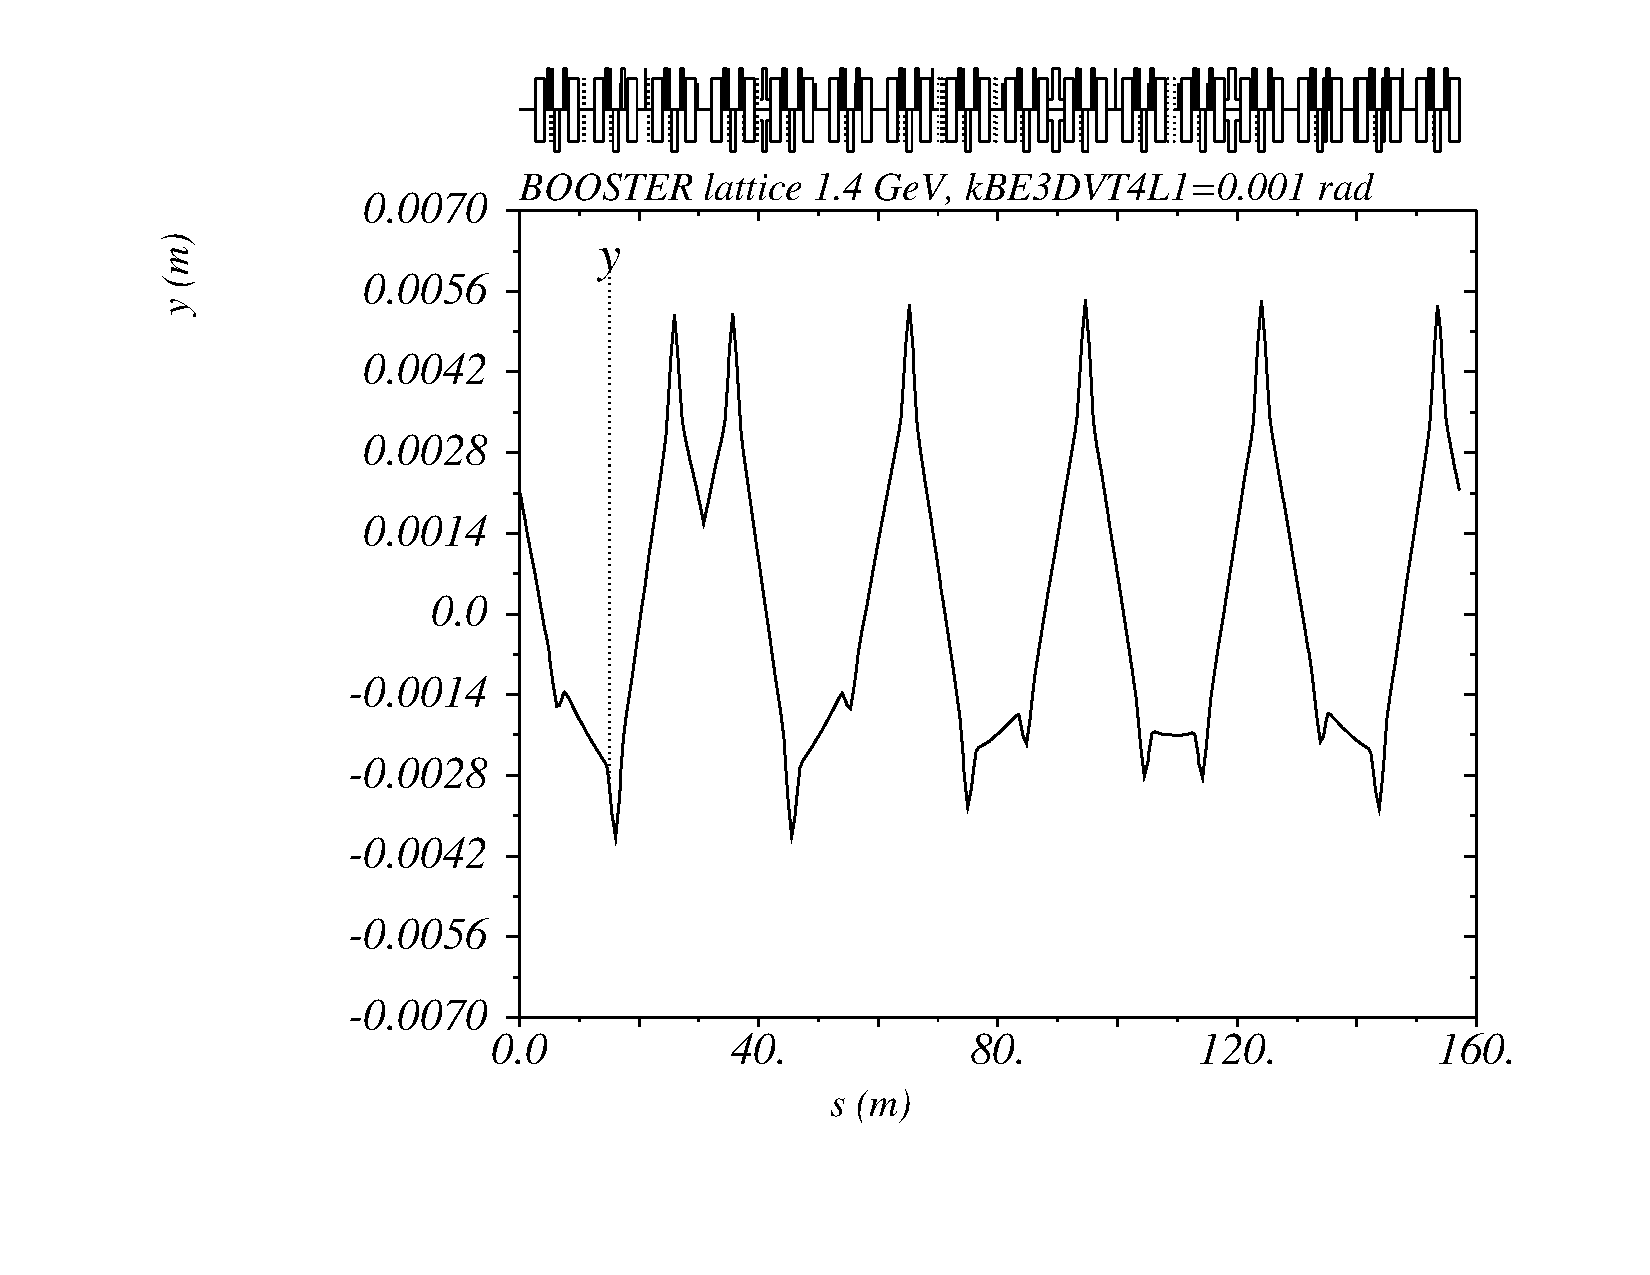
\includegraphics[width=1.0\textwidth]{figs/psb_orbit_BE3DVT4L1at1mrad.pdf}
%    \caption{Closed Orbit comparison for a kick of 1 mrad for BE3.DVT4L1. Top: from the note PS/OP/Note 99-xx of M. Benedikt. Bottom: Private MADX files}
%    \label{fig:BE_DVT4L1}
%  \end{center}
%\end{figure}
%
%
%\begin{figure}[!hbtp]
%  \begin{center}
%    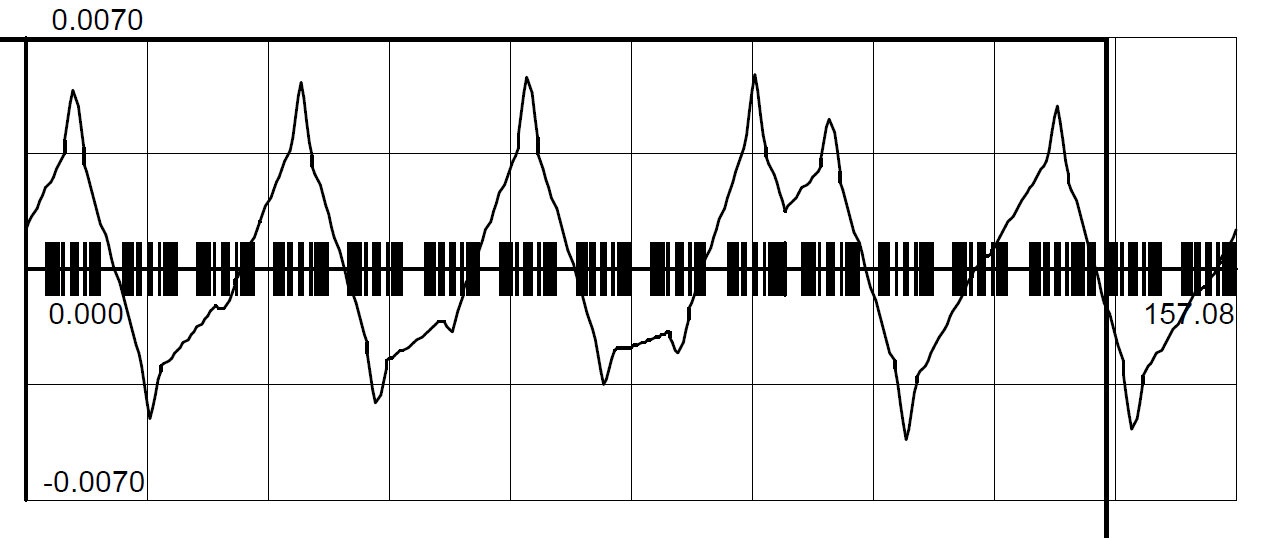
\includegraphics[width=1.0\textwidth]{figs/LINC-BE_DVT11L1.png}
%    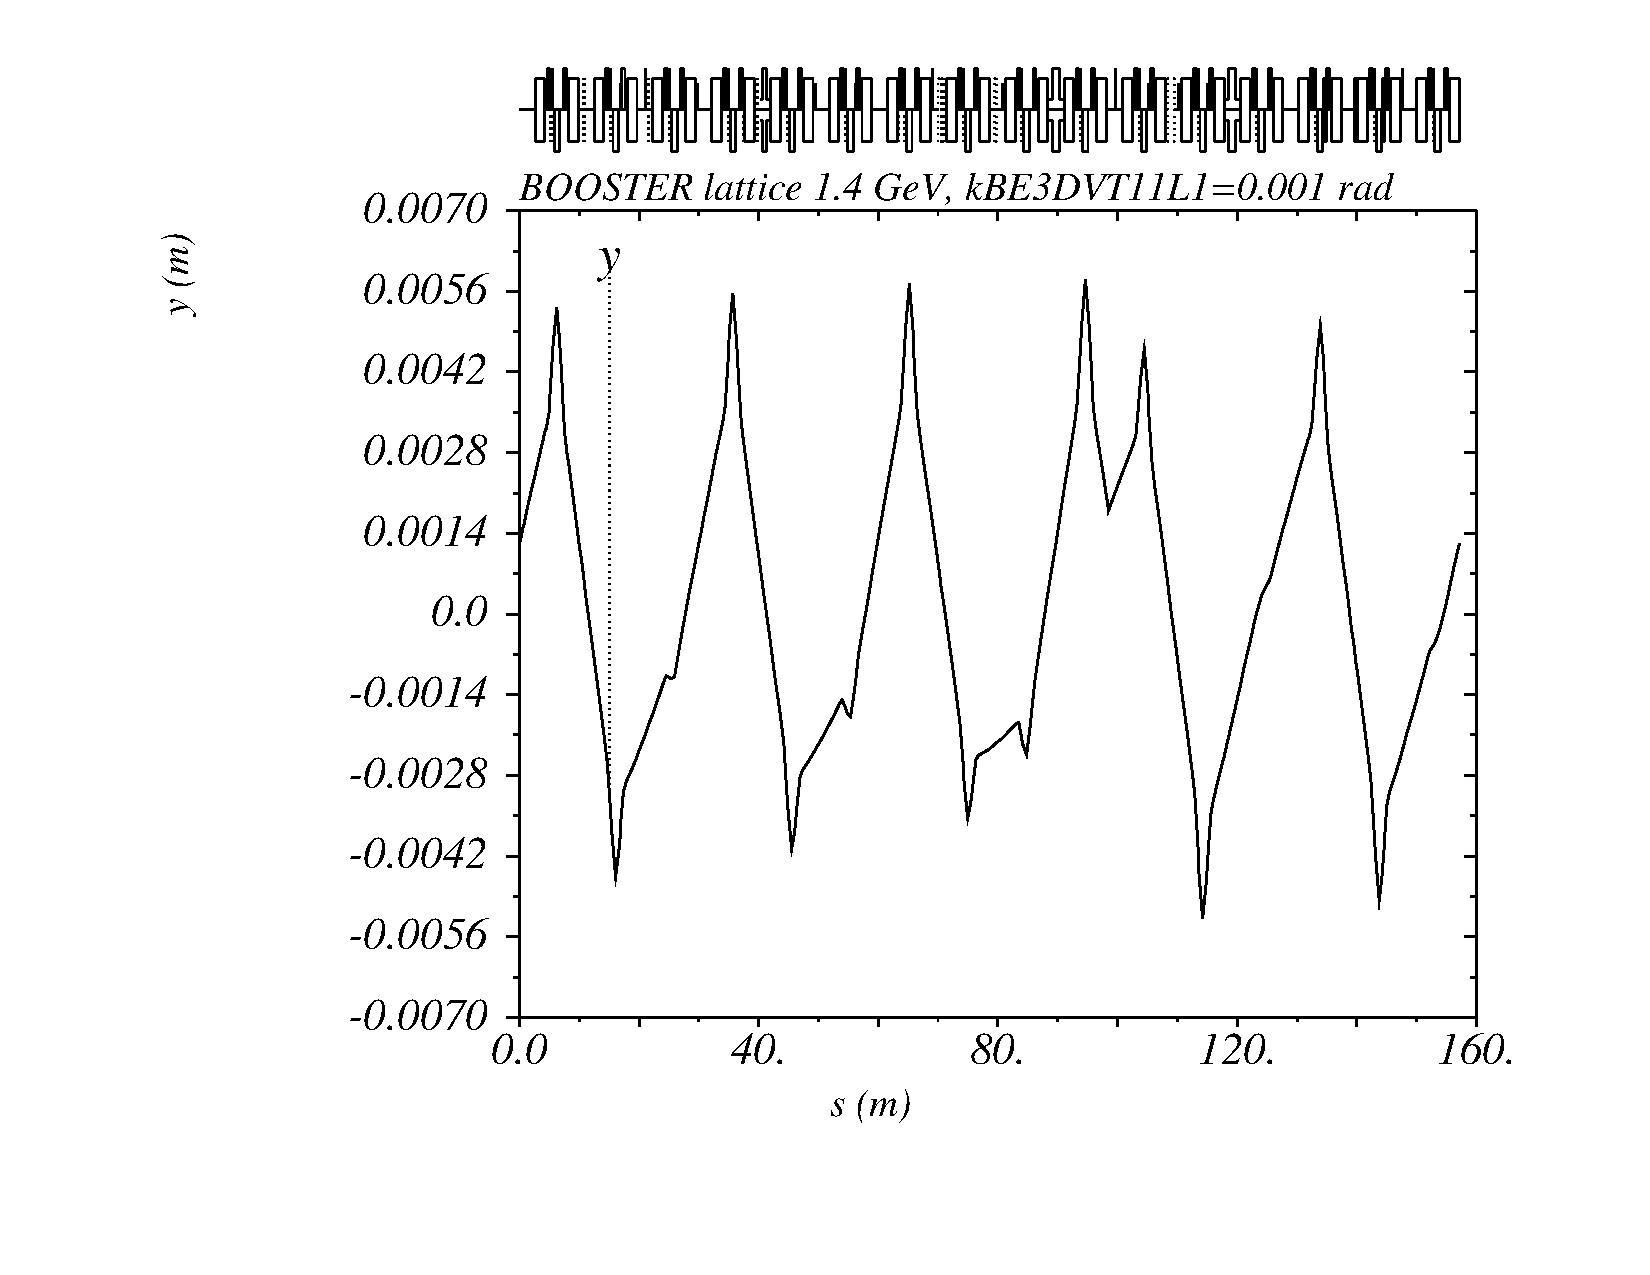
\includegraphics[width=1.0\textwidth]{figs/psb_orbit_BE3DVT11L1at1mrad.pdf}
%    \caption{Closed Orbit comparison for a kick of 1 mrad for BE3.DVT11L1. Top: from the note PS/OP/Note 99-xx of M. Benedikt. Bottom: Private MADX files}
%    \label{fig:BE_DVT11L1}
%  \end{center}
%\end{figure}
%
%
%
%%===============================================================================
%% To Do
%%===============================================================================
%\subsection*{Questions}
%
%\begin{itemize}
%\item{Do the results change for the 4 rings? {\bf No, is it expected?}}
%\item{Does the position of the kicker matter? {\bf Yes. E.g., by moving DHZ4L1 4 cm towards the beam I get much closer values of the ones in the note.}}
%\item{Which is the desired level of agreement? {\bf To be discussed with Bettina/Vivien. It is difficult for me to judge without errors associated to estimations}}
%\item{Where to estimate the geometrical relations? {\bf the note says ``entrance of the ejection septum'', although I think they used the center. I tried at the beginning of SMH15L1, but got not compatible values}}
%\end{itemize}





\end{document}


